\chapter{Alternative compositions}
\label{sec:comps}

Up until this point we have looked in detail at the high-entropy silicide \ch{(CrFeMnNi)Si2}. In this chapter we will broaden our search of compositions based on the $\beta-$ \ch{FeSi2} structure. First, we will look at various compositions inside the quaternary phase diagram of Cr, Fe, Mn and Ni, followed by compositions where chromium, manganese or nickel are replaced by cobalt or titanium. 

\section{Exploring the quaternary phase diagram}
In this section, we aim to expand our search of this diagram by generating SQSs of the 48 atom model slightly away from equimolar distribution of 3d elements. The compositions we test are listed in table 8.1, with corresponding total energy, magnetic moment and formation energy in the familiar format. Ideally each composition would differ only by one element to provide a clear view of each direction in the phase diagram, but the TDEP implementation insist in reducing Nickel to stay consistent with the 48 atom supercell. 

\begin{table}[H]
\centering
\begin{tabular}{@{}cccccc@{}}
\toprule
Composition           & \multicolumn{2}{c}{\begin{tabular}[c]{@{}c@{}}Toten\\ (eV)\end{tabular}} & \multicolumn{2}{c}{\begin{tabular}[c]{@{}c@{}}Mag \\ ($\mu_B$) \end{tabular}} & \begin{tabular}[c]{@{}c@{}}$E_{FPA}$\\ (eV) \end{tabular} \\ \midrule
                      & mean                                 & std                               & mean                                 & std                                 & mean                                                      \\ \midrule
\ch{Cr3Fe3Mn7Ni3Si32} & - 6.6947                             & 0.0040                            & 0.1375                               & 0.0186                              & -0.300                                                  \\
\ch{Cr5Fe5Mn3Ni3Si32} & - 6.6705                             & 0.0030                            & 0.1127                               & 0.0223                              & -0.286                                                  \\
\ch{Cr5Fe3Mn5Ni3Si32} & - 6.6852                             & 0.0041                            & 0.1375                               & 0.0456                              & -0.271                                                  \\
\ch{Cr3Fe5Mn5Ni3Si32} & - 6.6801                             & 0.0036                            & 0.0937                               & 0.0209                              & -0.315                                                  \\
\ch{Cr3Fe3Mn3Ni7Si32} & - 6.3921                             & 0.0078                            & 0.0159                               & 0.0101                              & -0.285                                                  \\ \bottomrule
\end{tabular}
\caption{Summary composition diagram}
\end{table}


In table 8.1 we observe that moving away from the equimolar system result in both less and more stable alloys. Clearly the most lowest formation energies (most stable) correspond to compositions rich in manganese and poor in chromium. Likewise the least stable compositions in table 8.1 contain either increased amounts of Cr or reduced amounts of Mn compared to the equimolar system. In the equimolar composition the magnetic moment was attributed to primarily Cr and Mn atoms in the lattice. In table 8.1 we observe similarly that compositions rich in Cr and Mn exhibits the largest magnetic moments and vice versa. The band gaps of the respective compositions in five unique SQSs can be seen in table 8.2 below, calculated with PBE GGA.   

\begin{table}[H]
\centering
\begin{tabular}{@{}ccccc@{}}
\toprule
Composition                                                 & SQS        & \begin{tabular}[c]{@{}c@{}}$E_G ^\text{up, eigen}(0.5)$\\ (eV)\end{tabular} & \begin{tabular}[c]{@{}c@{}}$E_G ^\text{dw, eigen}(0.5)$\\ (eV)\end{tabular} & \begin{tabular}[c]{@{}c@{}}$E_G ^\text{tot, eigen}(0.5, 0.5)$\\ (eV)\end{tabular} \\ \midrule
\multicolumn{1}{c|}{\multirow{5}{*}{\ch{Cr3Fe3Mn7Ni3Si32}}} & A          & 0.3390                                                                      & 0                                                                           & 0                                                                                 \\
\multicolumn{1}{c|}{}                                       & \textbf{B} & 0.4745                                                                      & 0                                                                           & 0                                                                                 \\
\multicolumn{1}{c|}{}                                       & C          & 0.1342                                                                      & 0                                                                           & 0                                                                                 \\
\multicolumn{1}{c|}{}                                       & D          & 0.1950                                                                      & 0.0063                                                                      & 0.0063                                                                            \\
\multicolumn{1}{c|}{}                                       & E          & 0.4211                                                                      & 0                                                                           & 0                                                                                 \\ \midrule
\multicolumn{1}{c|}{\multirow{4}{*}{\ch{Cr5Fe5Mn3Ni3Si32}}} & A          & \textit{0.003}                                                              & 0                                                                           & 0                                                                                 \\
\multicolumn{1}{c|}{}                                       & \textbf{C} & \textit{0.21}                                                               & 0                                                                           & 0                                                                                 \\
\multicolumn{1}{c|}{}                                       & D          & 0.0674                                                                      & 0.0413                                                                      & 0.0372                                                                            \\
\multicolumn{1}{c|}{}                                       & E          & \textit{0.362}                                                              & 0                                                                           & 0                                                                                 \\ \midrule
\multicolumn{1}{c|}{\multirow{5}{*}{\ch{Cr5Fe3Mn5Ni3Si32}}} & \textbf{A} & 0.2082                                                                      & 0                                                                           & 0                                                                                 \\
\multicolumn{1}{c|}{}                                       & B          & 0.4053                                                                      & 0                                                                           & 0                                                                                 \\
\multicolumn{1}{c|}{}                                       & C          & 0.4659                                                                      & 0                                                                           & 0                                                                                 \\
\multicolumn{1}{c|}{}                                       & D          & 0.0843                                                                      & 0.0121                                                                      & 0.0121                                                                            \\
\multicolumn{1}{c|}{}                                       & E          & 0.3008                                                                      & 0                                                                           & 0                                                                                 \\ \midrule
\multicolumn{1}{c|}{\multirow{4}{*}{\ch{Cr3Fe5Mn5Ni3Si32}}} & A          & 0.3922                                                                      & 0                                                                           & 0                                                                                 \\
\multicolumn{1}{c|}{}                                       & C          & 0.1285                                                                      & 0                                                                           & 0                                                                                 \\
\multicolumn{1}{c|}{}                                       & \textbf{D} & 0.2595                                                                      & 0.1004                                                                      & 0.1004                                                                            \\
\multicolumn{1}{c|}{}                                       & E          & 0.3591                                                                      & 0.1003                                                                      & 0.0848                                                                            \\ \midrule
\multicolumn{1}{c|}{\multirow{5}{*}{{Cr3Fe3Mn3Ni7Si32}}}    & A          & 0                                                                           & 0                                                                           & 0                                                                                 \\
\multicolumn{1}{c|}{}                                       & B          & 0                                                                           & 0                                                                           & 0                                                                                 \\
\multicolumn{1}{c|}{}                                       & C          & 0                                                                           & 0                                                                           & 0                                                                                 \\
\multicolumn{1}{c|}{}                                       & D          & 0                                                                           & 0                                                                           & 0                                                                                 \\
\multicolumn{1}{c|}{}                                       & \textbf{E} & \textit{0.04}                                                               & 0                                                                           & 0                                                                                 \\ \bottomrule 
\end{tabular}
\caption{Band gaps of various compositions of \ch{(CrFeMnNi)Si2}. Most stable SQS of a set is highlighted in bold text, defect/impurity band gap are listed in cursive. Some SQSs were excluded from the table due to unsuccessful calculations.}
\end{table}

From table 8.2 we observe that most compositions are half-metals alike the equimolar system with a spin up polarization. Each composition show large variation between configurations. We note $E_\text{G, max} ^\text{up} \approx 0.5$ eV and $E_\text{min} ^\text{up} \approx 0.1$ eV in both \ch{Cr3Fe3Mn7Ni3Si32} and \ch{Cr5Fe3Mn5Ni3Si32}, and further $E_\text{G, max} ^\text{up} \approx 0.4$ eV and $E_\text{min} ^\text{up} \approx 0.1$ eV in \ch{Cr3FeMn5Ni3Si32}. In all three of these compositions the proportion of manganese is increased relative to the equimolar system, and two out of the three compositions contain reduced amounts of chromium. Looking at the two compositions with the least indication of a band gap \ch{Cr5Fe5Mn3Ni3Si32} and \ch{Cr3Fe3Mn3Ni7}, these contain reduced amounts of manganese. Thus, based on the few compositions tested in this experiment we can state a relation of the band gap mainly to manganese, but also chromium.     

Based on the utmost stable configuration of each composition, we observe very encouraging results in the \ch{Cr3Fe3Mn7Ni3Si32} composition with the largest $E_G ^\text{up}$ of the set of configurations, likewise the most stable SQS of the \ch{Cr3Fe5Mn5Ni3Si32} composition is a semiconductor with a total band gap of about 0.1 eV. In the composition \ch{Cr5Fe5Mn3Ni3Si32} the most stable SQS predicts a defect or impurity band gap as we discussed previously where the eigenvalues return a finite band gap despite of defect states. However we have not been able to investigate the nature and effect of this impurity band gap to further extent, likewise for the similar impurity gaps listed in table 8.2 and the 0 band gaps in spin down. Below in figures 8.1 and 8.2 we include the projected density of states around $E_F$ of the utmost stable SQS of each composition. Becouse we only include and discuss the most stable SQS, the features of these figures can be subject to the uniqueness of that particular SQS rather than a distinct feature of the exact composition, but as stated previously the most stable configuration provide the most likely properties of the composition within the scope of this project. 

\begin{figure}[H]
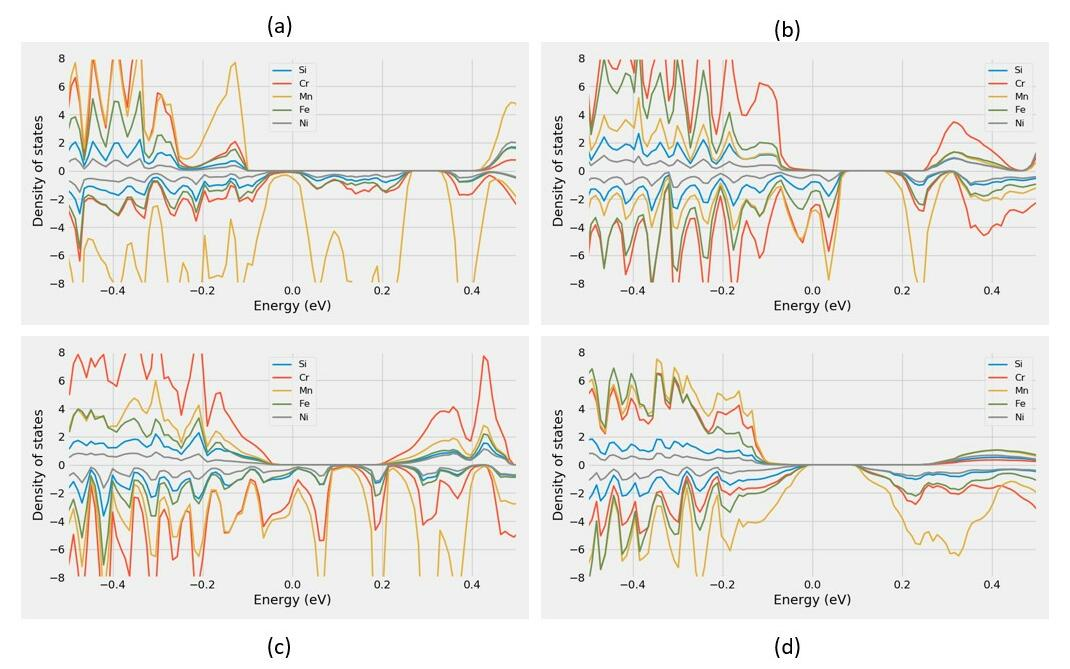
\includegraphics[width=\linewidth]{results/fesi2/permutations/perm_LDOS_crop.jpg}
\caption{Projected density of states of (a) \ch{Cr3Fe3Mn7Ni3Si32} (SQS B), (b) \ch{Cr5Fe5Mn3Ni3Si32} (SQS C), (c) \ch{Cr5Fe3Mn5Ni3Si32} (SQS A), (d) \ch{Cr3Fe5Mn5Ni3Si32} (SQS D)}
\end{figure}

The PDOSs is in good agreement with the listed values in table 7.2. \ch{Cr3Fe3Mn7Ni3Si32}  and \ch{Cr5Fe3Mn5Ni3Si32} both display sizable band gaps in spin, while figure 8.1 d point to a total band gap around 0.1 eV for SQS D of \ch{Cr3Fe5Mn5Ni3Si32}. On the other hand we observe as for the 192-atom SQS a dissimilarity between the density of states band gap in \ch{Cr5Fe5Mn3Ni3Si32} SQS C (figure 8.1 b) and the eigenvalue (impurity) band gap listed in table 7.2. This can be better understood by figure .. in appendix .. that display a zoomed in DOS that clearly show small finite values at $E_F$ in spin up. This DOS may resemble that of a n-doped material where the Fermi energy is pushed up in energy.    


In figure 7.7 we saw that manganese distinctly occupied states in the spin down channel around $E_F$ and was a key contributor as to why the spin down channel of \ch{(CrFeMnNi)Si2} was metallic in the utmost stable SQS. This is also largely the case in the compositions shown above in figure 8.1 and 8.2, and is particularly evident in figure 8.1 where Mn dominate the spin down states around $E_F$ in the \ch{Cr3Fe3Mn7Ni3Si32} composition. By reducing the number of Mn we still find that the Mn states prohibit the band gap in spin down, as seen in figure 8.1 b. In the chromium rich compositions plotted in figures 8.1 b and c, we observe that also Cr states prohibit the spin down band gap, and dominate states near $E_F$ in spin up as well. Contrary, in the \ch{Cr3Fe3Mn3Ni7Si32} composition plotted in figure 8.2, we do not observe any distinct peaks of elements, but rather consistent small finite DOS around $E_F$ in all elements.  The sole composition with clear evidence of a spin down gap is from the chromium poor system plotted in figure 8.1 d. Also in this structure we see that the effects of Mn around $E_F$ is dominant in spin down from the relative large amounts of Mn, but in comparison to the other composition these states are pushed away from the Fermi energy.

\begin{figure}[H]
	\centering
	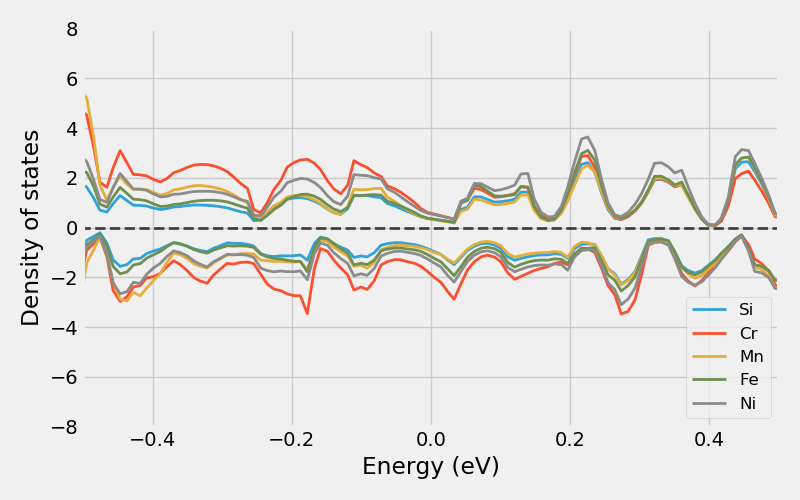
\includegraphics[width=.6\textwidth]{results/fesi2/permutations/ni7_PDOS.png}
	\caption{Projected density of states of \ch{Cr3Fe3Mn3Ni7Si32} around $E_F$}
\end{figure}

An important factor of these results is that because each composition alters simultaneous elements, interpreting and relating the results to a particular alteration is challenging. For example, is the result of the \ch{Cr5Fe3Mn5Ni3Si32} permutation a consequence of less Fe or increments to both Cr and Mn? Furthermore is the large band gap in spin up of \ch{Cr3Fe3Mn7Ni3Si32} a product of increasing manganese or reducing the other elements. From the comparatively large gaps in spin up of \ch{Cr3Fe3Mn7Ni3Si32} and \ch{Cr3Fe5Mn5Ni3Si32} and the more present Cr states in spin up in the Cr rich permutations we here conclude that the band gap is related to lessening of chromium, more so than other effects. However we see from both \ch{Cr5Fe5Mn4Ni3Si32} and \ch{Cr3Fe3Mn3Ni7Si32} (figure 8.2) in addition to the manganese rich composition that Mn plays a vital role on the band gap of these structures. It's clear that the \ch{Cr3Fe5Mn5Ni3Si32} alloy manage to strike a balance between 3d elements that results in a specific interplay and correspondingly very promising properties. It would have been beneficiary to look at for example the pair distribution functions and compare to the equimolar system, but from the factors discussed in section 7.2.4 we leave this to future work. 

As stated before, we relied on the PBE GGA functional to determine the band gap in this part from its reliability and favorably computation cost. However we have conducted calculations with SCAN and HSE06 on some of the more promising structures. For instance in SQS D of \ch{Cr3Fe5Mn5Ni3Si32} we get lower values in both spin up and down with SCAN, specifically $E_\text{G, SCAN} ^\text{up}= 0.21$ eV and $E_\text{G, SCAN} ^\text{dw} = 0.08$ eV, and on the other hand HSE06 predicts $E_\text{G, HSE06} ^\text{up} = 0.53$ eV and $E_\text{G, HSE06} ^\text{dw} = 0$ eV. In SQS B of \ch{Cr3Fe3Mn7Ni3Si32} we observe very different outcomes. With SCAN we get a small band gap in spin down of about 0.002 eV and 0 in spin up, likewise the HSE06 band gap of this structure is $E_\text{G, HSE06} ^\text{up} = 0.08$ eV and $E_\text{G, HSE06} ^\text{dw} = 0.11$ eV, opposed to $E_\text{G, PBE} ^\text{up} = 0.47$ eV and $E_\text{G, PBE} ^\text{dw} = 0$ eV. Further the HSE06 band gap is in fact an impurity band gap, with $E_\text{G, HSE06} ^\text{up, eigen}(0.01) = 0.18$ eV and $E_\text{G, HSE06} ^\text{dw, eigen}(0.01) = 0.16$ eV.


\section{High entropy silicides with cobalt/titanium}

In similar fashion to the preceding section, we begin by presenting the new high-entropy silicides by the mean and standard deviation of the total energy and magnetization of 5 unique SQSs of each alloy in table 8.3. The compositions we have tested are deliberate combinations intended to investigate the role elements in the \ch{(CrFeMnNi)Si2} system, by introducing Co/Ti at the cost of different elements. Note that the alloys contain a total of 48 atoms as before, based on the $\beta-$ \ch{FeSi2} unit cell and equimolar distribution of 3d elements.   

\begin{table}[H]
\centering
\begin{tabular}{@{}cccccc@{}}
\toprule
Composition           & \multicolumn{2}{c}{\begin{tabular}[c]{@{}c@{}}Toten \\ (eV)\end{tabular}} & \multicolumn{2}{c}{\begin{tabular}[c]{@{}c@{}}Mag\\ ($\mu_B$)\end{tabular}} & \begin{tabular}[c]{@{}c@{}}$E_{FPA}$\\ (eV)\end{tabular} \\ \midrule
                      & mean                                 & std                                & mean                                 & std                                  & mean                                                      \\ \midrule
\ch{Cr4Fe4Co4Ni4Si32} & - 6.4655                             & 0.0056                             & 0.0083                               & 0.0155                               & -0.308                                                 \\
\ch{Co4Fe4Mn4Ni4Si32} & - 6.4731                             & 0.0046                             & 0.0000                               & 0.0000                               & -0.355                                                 \\
\ch{Cr4Fe4Ti4Ni4Si32} & - 6.4217                             & 0.0087                             & 0.0305                               & 0.0293                               & -0.209                                                  \\
\ch{Cr4Fe4Mn4Ti4Si32} & -6.6994                              & 0.0071                             & 0.1142                               & 0.0641                               & -0.199                                                  \\
\ch{Cr4Fe4Mn4Co4Si32} & -6.7687                              & 0.0034                             & 0.1331                               & 0.0326                               & -0.323                                                  \\ \bottomrule
\end{tabular}
\caption{Overview new compositions}
\end{table}

In terms of the formation energy, we observe that cobalt evidently yield the utmost stable alloys from the tested compositions, with \ch{(CoFeMnNi)Si2} at the top and and \ch{(CrFeCoNi)Si2} at the bottom. On the other side, both \ch{(CrFeTiNi)Si2} and \ch{(CrFeMnTi)Si2} where we introduce titanium in place of manganese and nickel respectively, result in the overall least stable compositions. A precise physical interpretation of the stability between compositions is challenging from the shallow analysis in this project, but we do note that the two most stable alloys consist of the most chemically similar elements with respect to of properties such as the electronegativity and atomic size. Following the least stable alloys are comprised of the most chemically dissimilar elements. This is in good agreement with the discussion in section 2.2 regarding phase formation of high-entropy alloys. Additionally, in the compositions discussed in the previous section we found that the most stable composition was \ch{Cr3Fe5Mn5Ni3Si32} where the Cr proportion was lessened. In conjunction with the results of the titanium we thus may suspect that smaller elements are ill-suited in this structure.   

In line with the other compositions studied in this project, the magnetization is clearly related to chromium and manganese also in this case. This is seen by the overall lowest magnetic moments in the two compositions without these elements, and reversely the highest magnetic moments is found for compositions with both Cr and Mn. Comparing the magnetic moment of \ch{(CrFeCoNi)Si2} and \ch{(CoFeMnNi)Si2} it seems in our study that chromium is most responsible for the magnetic moment in these alloys. Furthermore we find that substituting Ni with both Ti and Co yields more magnetic compounds. As we have discussed previously, the uniqueness of each SQS makes it difficult to draw conclusion on the various properties. In table 8.4 below we list the magnetic moment of the utmost stable SQS in each alloy. Contrary to the mean value we find that \ch{(CrFeCoNi)Si2} equal to \ch{(CoFeMnNi)Si2} is nonmagnetic, moreover \ch{(CrFeMnTi)Si2} are less magnetic relative to both \ch{(CrFeMnCo)Si2} and \ch{(CrFeMnNi)Si2}. 

\begin{table}[H]
\centering
\begin{tabular}{@{}lc@{}}
\toprule
\multicolumn{1}{c}{Composition} & \begin{tabular}[c]{@{}c@{}}Magnetic moment\\ ($\mu_B$)\end{tabular} \\ \midrule
\ch{Cr4Fe4Co4Ni4Si32}           & 0                                                                   \\
\ch{Co4Fe4Mn4Ni4Si32}           & 0                                                                   \\
\ch{Cr4Fe4Ti4Ni4Si32}           & 0,0653                                                              \\
\ch{Cr4Fe4Mn4Ti4Si32}           & 0,0785                                                              \\
\ch{Cr4Fe4Mn4Co4Si32}           & 0,1666                                                              \\ \bottomrule
\end{tabular}
\caption{Final magnetic moment of the utmost stable SQS of each composition.}
\end{table}

Thus, based on the utmost stable configurations we can state that replacing either Cr or Mn (with Co), removes the magnetic moment of the alloy. Furthermore we find that the magnetic moment is reduced when Ni is substituted with Ti, and increased by Co. However, while substituting manganese with Co yields a nonmagnetic alloy, Ti for Mn only slightly reduces the magnetic moment. 

In regards to the band gap, we find most to be metals. In table 8.5 we list the band gap of the utmost stable SQS of each composition, where the band gap is determined from the eigenvalues at different occupancy cutoff $occ$ values to underline the effect of defect states. We find that increasing the criteria, in other words only consider states with occupancy above a certain threshold, the band gap become finite with $occ = 0.1$ and converge to around $0.02 - 0.06$ eV depending on composition at $occ = 0.01$ and beyond.

\begin{table}[H]
\centering
\begin{tabular}{@{}ccccc@{}}
\toprule
\multicolumn{1}{l}{Composition}                   & $occ$                     & \begin{tabular}[c]{@{}c@{}}$E_\text{G} ^\text{up, eigen}$\\ (eV)\end{tabular} & \begin{tabular}[c]{@{}c@{}}$E_\text{G} ^\text{dw, eigen}$\\ (eV)\end{tabular} & \begin{tabular}[c]{@{}c@{}}$E_\text{G} ^\text{tot, eigen}$\\ (eV)\end{tabular} \\ \midrule
\multicolumn{1}{c|}{\multirow{3}{*}{\ch{CrFeCoNiSi2}}}                  & \multicolumn{1}{c|}{0.5}  & 0                                                                             & 0                                                                             & 0                                                                              \\
\multicolumn{1}{c|}{}                             & \multicolumn{1}{c|}{0.1}  & 0.00095                                                                       & 0.0399                                                                        & 0.00095                                                                        \\
\multicolumn{1}{c|}{}                             & \multicolumn{1}{c|}{0.01} & 0.063                                                                         & 0.063                                                                         & 0.063                                                                          \\ \midrule
\multicolumn{1}{c|}{\multirow{3}{*}{\ch{CrFeTiNiSi2}}} & \multicolumn{1}{c|}{0.5}  & 0.0067                                                                        & 0                                                                             & 0                                                                              \\
\multicolumn{1}{c|}{}                             & \multicolumn{1}{c|}{0.1}  & 0.061                                                                         & 0.0087                                                                        & 0.0087                                                                         \\
\multicolumn{1}{c|}{}                             & \multicolumn{1}{c|}{0.01} & 0.061                                                                         & 0.037                                                                         & 0.037                                                                          \\ \midrule
\multicolumn{1}{c|}{\multirow{3}{*}{\ch{CoFeMnNiSi2}}} & \multicolumn{1}{c|}{0.5}  & 0                                                                             & 0                                                                             & 0                                                                              \\
\multicolumn{1}{c|}{}                             & \multicolumn{1}{c|}{0.1}  & 0.0037                                                                        & 0.0037                                                                        & 0.0037                                                                         \\
\multicolumn{1}{c|}{}                             & \multicolumn{1}{c|}{0.01} & 0.0268                                                                        & 0.0268                                                                        & 0.0268                                                                         \\ \midrule
\multicolumn{1}{c|}{\multirow{3}{*}{\ch{CrFeMnTiSi2}}} & \multicolumn{1}{c|}{0.5}  & 0                                                                             & 0                                                                             & 0                                                                              \\
\multicolumn{1}{c|}{}                             & \multicolumn{1}{c|}{0.1}  & 0.021                                                                         & 0.00049                                                                       & 0                                                                              \\
\multicolumn{1}{c|}{}                             & \multicolumn{1}{c|}{0.01} & 0.03                                                                          & 0.03                                                                          & 0.022                                                                          \\ \midrule
\multicolumn{1}{c|}{\multirow{3}{*}{\ch{CrFeMnCoSi2}}} & \multicolumn{1}{c|}{0.5}  & 0.461                                                                         & 0                                                                             & 0                                                                              \\
\multicolumn{1}{c|}{}                             & \multicolumn{1}{c|}{0.1}  & 0.607                                                                         & 0.0218                                                                        & 0.0218                                                                         \\
\multicolumn{1}{c|}{}                             & \multicolumn{1}{c|}{0.01}                      & 0.607                                                                         & 0.0245                                                                        & 0.0245                                                                         \\ \bottomrule
\end{tabular}
\caption{The band gap in spin up/down and total of the utmost stable SQS in five high-entropy silicides based on $\beta$-\ch{FeSi2}}
\end{table}
 
The \ch{CrFeMnCoSi2} composition exhibits a band gap of around 0.5 eV in spin up, contrary to the metallic compositions. We observe that the gap similar to the \ch{Cr5Fe5Mn3Ni3Si32} composition and the the 192-atom SQS in section 7.2.5, is an impurity gap that contain a small number of defect states in addition to the finite gap. As was the case in these structures, the band gap in \ch{(CrFeMnCo)Si2} display small nonzero DOS at the Fermi energy, as seen from the projected density of states in figure 8.3. As observed in the previous compositions, the PDOS in this alloy point to a severe number of manganese states in spin down at energies just above $E_F$, and further large number of Cr states right below $E_F$ in spin up.  
  
\begin{figure}[H]
\centering
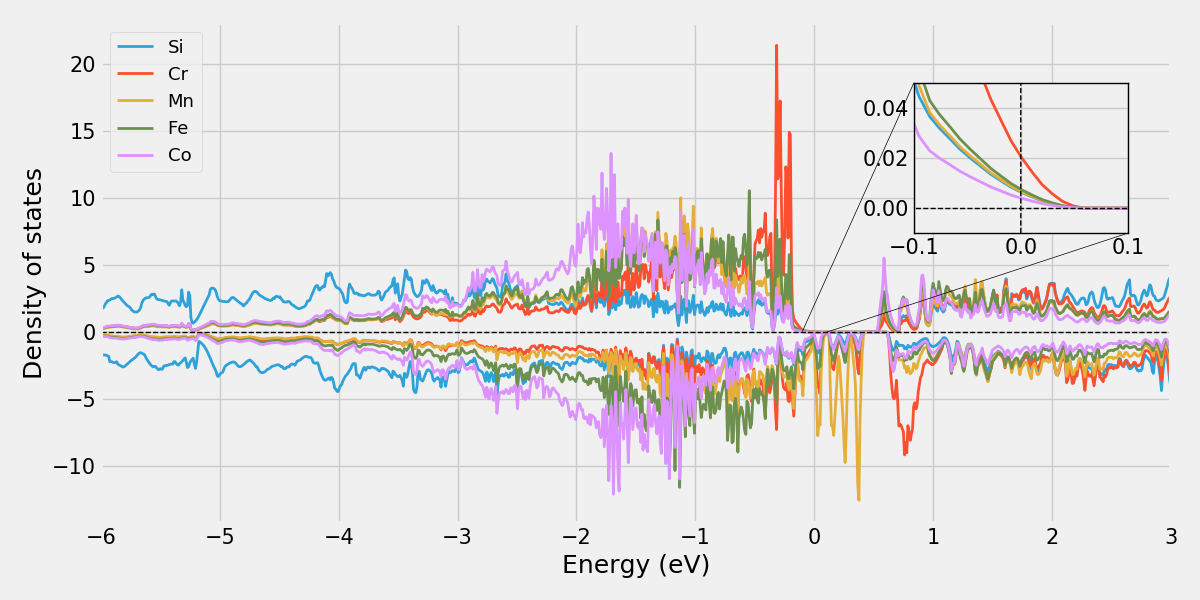
\includegraphics[width=\textwidth]{results/fesi2/composistions/crfemnco_PDOS.png}
\caption{Projected density of states of \ch{(CrFeMnCo)Si2}.}
\end{figure}

The PDOS of the other four alloys are included in figure 8.4 below. In agreement with the values listed in table 8.5 we observe clear indication of metallic structures, furthermore in agreement with the magnetic moments discussed previously. 

\begin{figure}[H]
\begin{subfigure}{.5\textwidth}
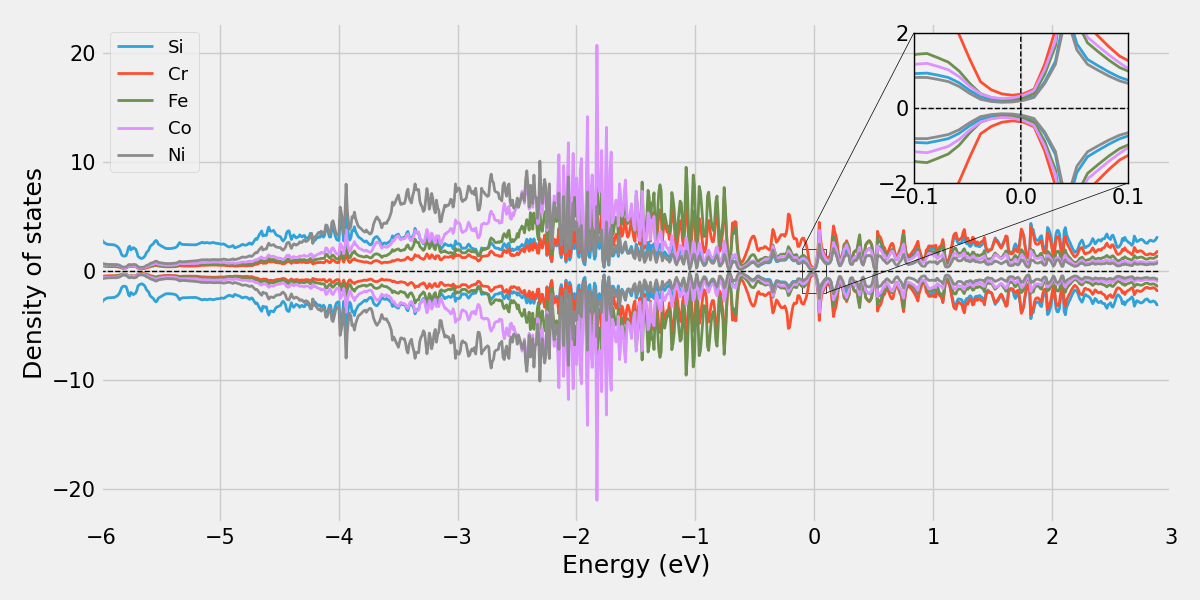
\includegraphics[width=\textwidth]{results/fesi2/crfeconi_PDOS.png}
\caption{\ch{Cr4Fe4Co4Ni4Si32}}
\end{subfigure}
\begin{subfigure}{.5\textwidth}
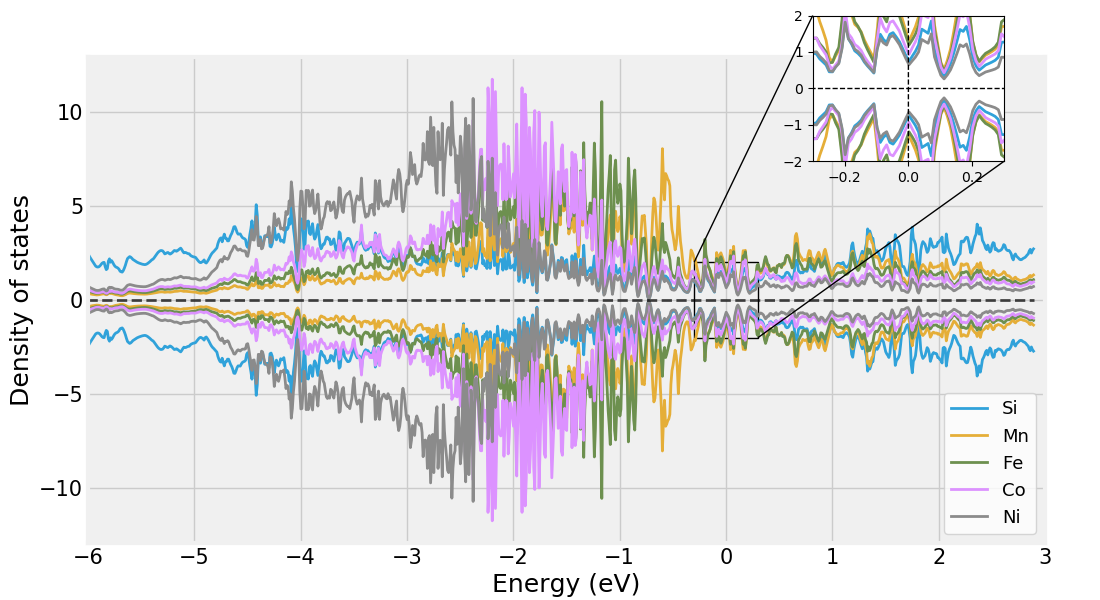
\includegraphics[width=\textwidth]{results/fesi2/cofemnni_PDOS.png}
\caption{\ch{Co4Fe4Mn4Ni4Si32}}
\end{subfigure}
\begin{subfigure}{.5\textwidth}
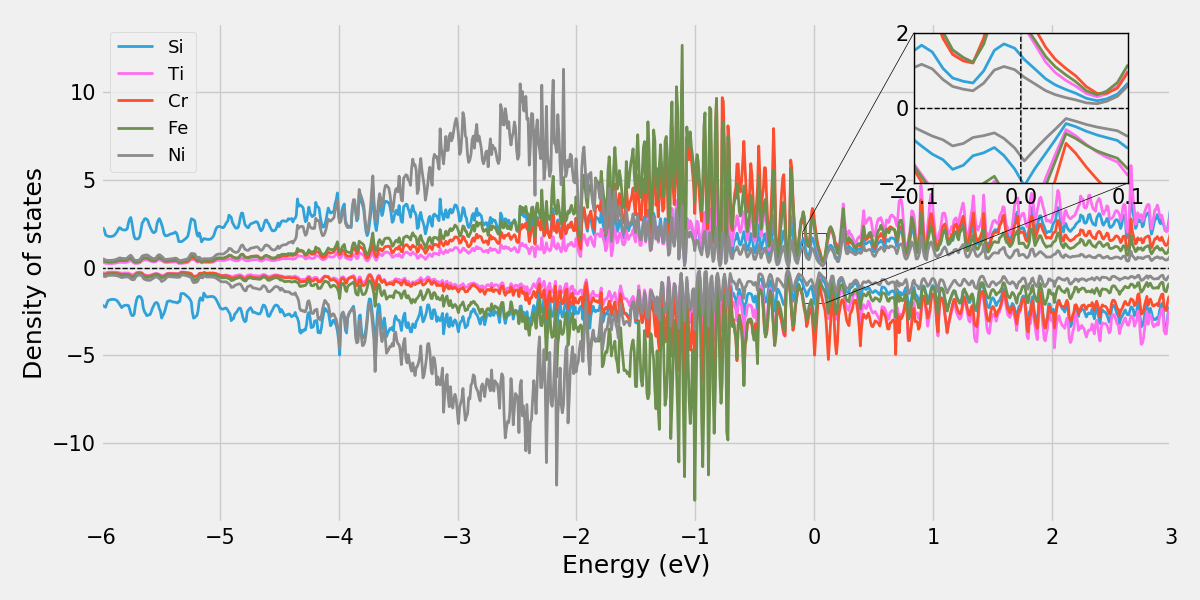
\includegraphics[width=\textwidth]{results/fesi2/crfetini_PDOS.png}
\caption{\ch{Cr4Fe4Ti4Ni4Si32}}
\end{subfigure}
\begin{subfigure}{.5\textwidth}
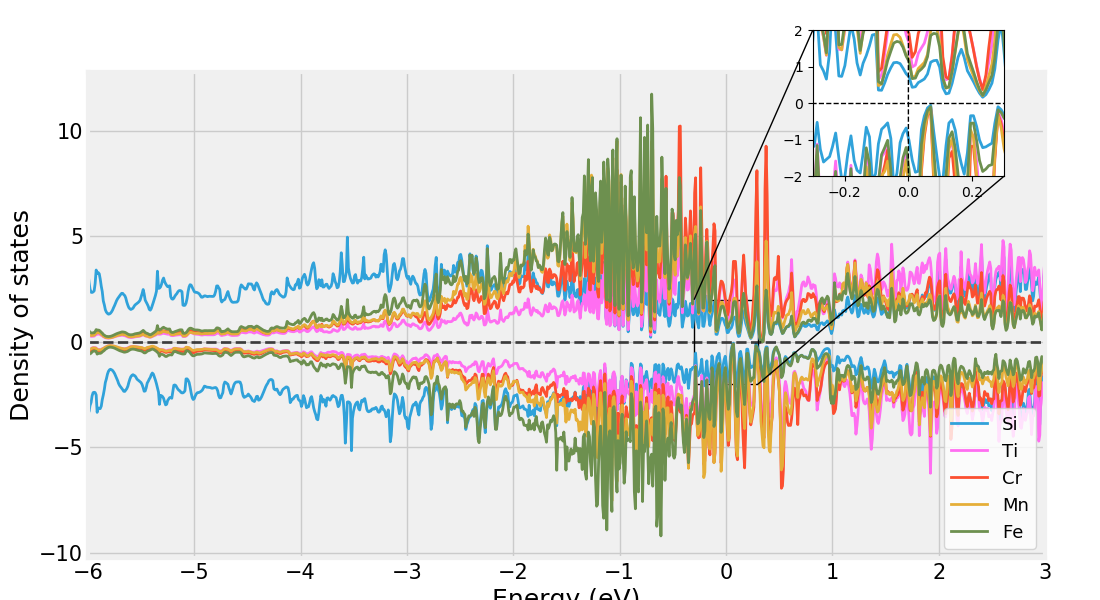
\includegraphics[width=\textwidth]{results/fesi2/crfemnti_PDOS.png}
\caption{\ch{Cr4Fe4Mn4Ti4Si32}}
\end{subfigure}
\caption{Projected density of states}
\end{figure}

Above we have evaluated the band gap of the different alloys based on the most stable configuration. Across all five configurations we find that the band gap is more or less consistent in \ch{(CrFeCoNi)Si2},  \ch{(CrFeMnTiSi2)}, \ch{(CrFeTiNi)Si2} and \ch{(CrFeMnCo)Si2}.  The most interesting case is the \ch{CoFeMnNiSi2} alloy, where we observed very narrow total band gaps in two lesser stable configurations (SQS A and E) of 0.03 eV and 0.006 eV respectively. Opposite of the impurity gaps discussed above, these are apparent in the density of states plots, as seen in figure 8.5 below. 

\begin{figure}[H]
\begin{subfigure}{.5\textwidth}
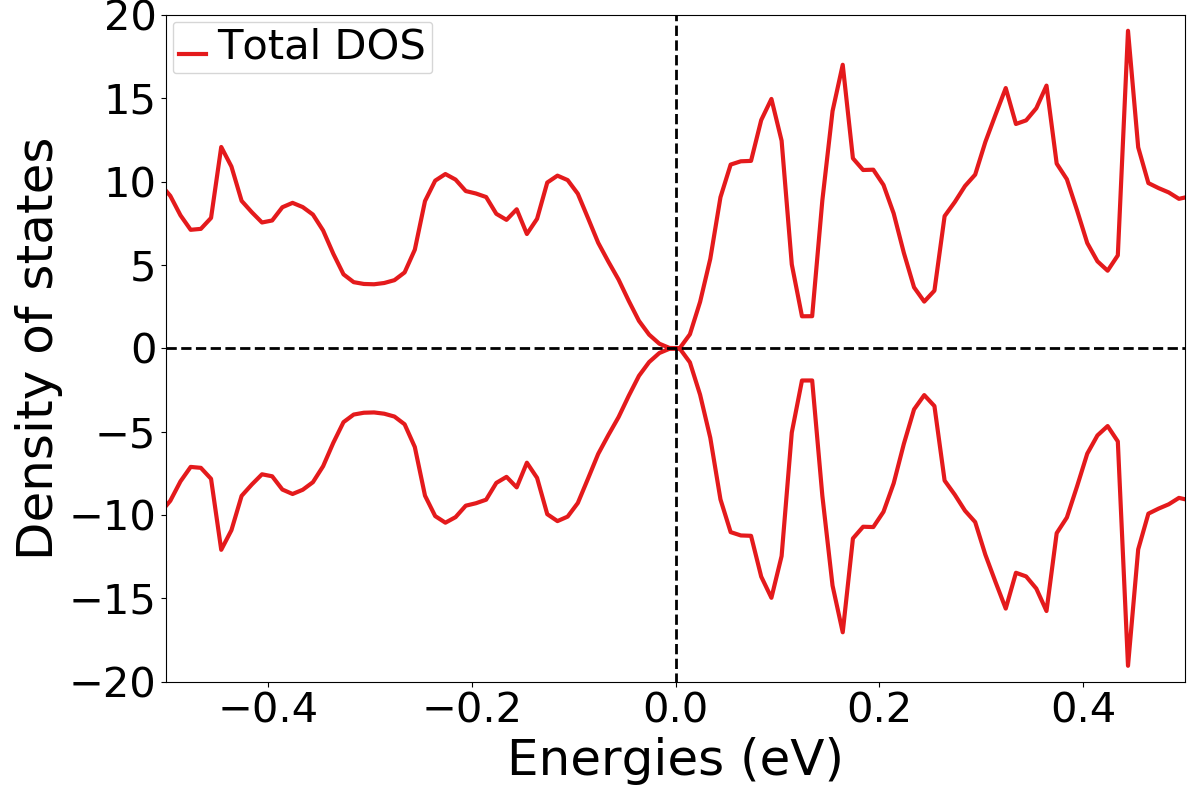
\includegraphics[width=\textwidth]{results/fesi2/composistions/cofemnni_E_DOS.png}
\caption{SQS A}
\end{subfigure}
\begin{subfigure}{.5\textwidth}
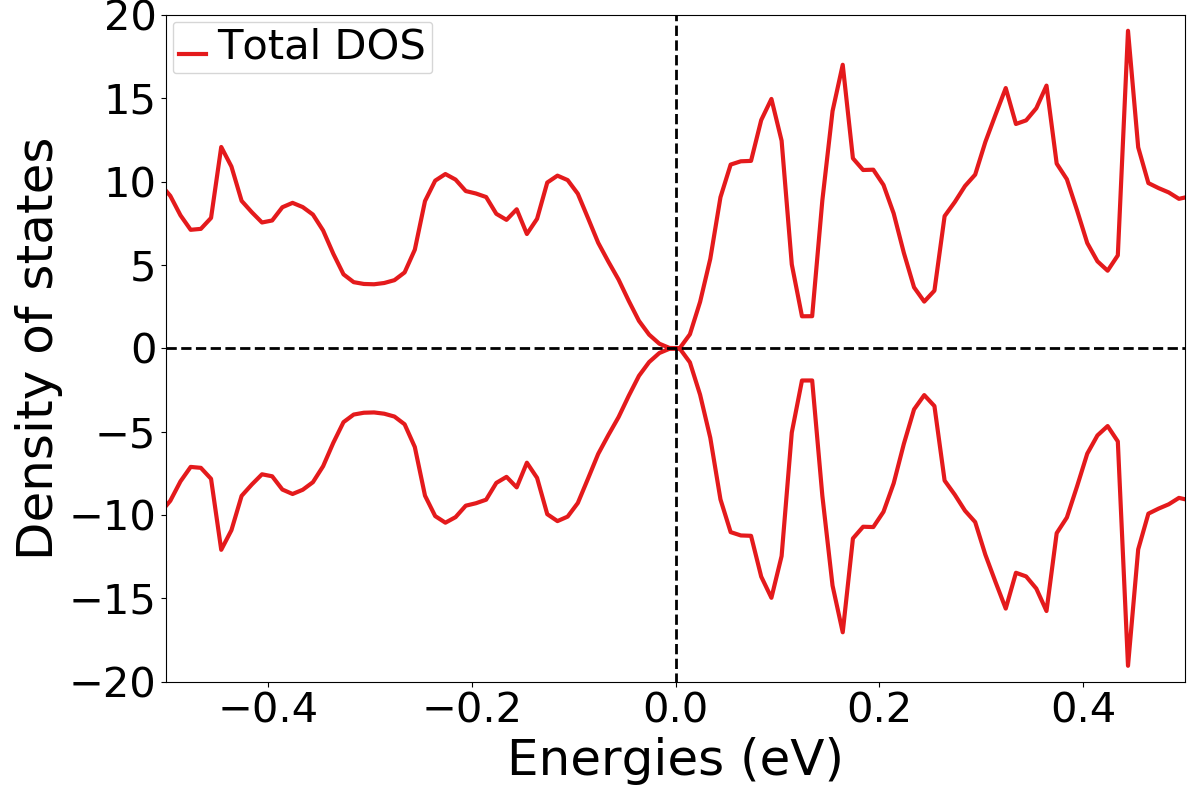
\includegraphics[width=\textwidth]{results/fesi2/composistions/cofemnni_E_DOS.png}
\caption{SQS E}
\end{subfigure}
\caption{Density of states of two SQS A and E of \ch{(CoFeMnNi)Si2}.}
\end{figure} 

In addition to the tests discussed above, we attempted to replicate the \ch{CrFeMnNi} system based on other silicides, such as hexagonal \ch{CrSi2}, trigonal \ch{Fe2Si}, and tetragonal and orthorombic \ch{Mn4Si7}, but found no indication of a band gap in these alloys. Furthermore we have tested a few alloys consisting of Sc, V, Zn, and Cu as well, but found no band gaps in these compositions either. 

